\makeatletter
\def\input@path{{../../}}
\makeatother
\documentclass[../../main.tex]{subfiles}

\graphicspath{
	{../../img/}
	{../img/}
	{img/}
}

\begin{document}
\section{Поверхности в $\R^3$}

Пусть в некоторой области $D \subset \R^2$ определены функции 
$x = x(u,v),\ y =y(u,v),\ z = \\ = z(u,v),\ (u,v) \in D$. 
Когда $(u,v)$ пробегает $D$, то в $\R^3$
определена некоторая поверхность $\Pi 
\iff$ задан вектор $\vec{r} = \vec{r}(u,v) = (x(u,v), y(u,v), z(u,v))$.

\begin{center}
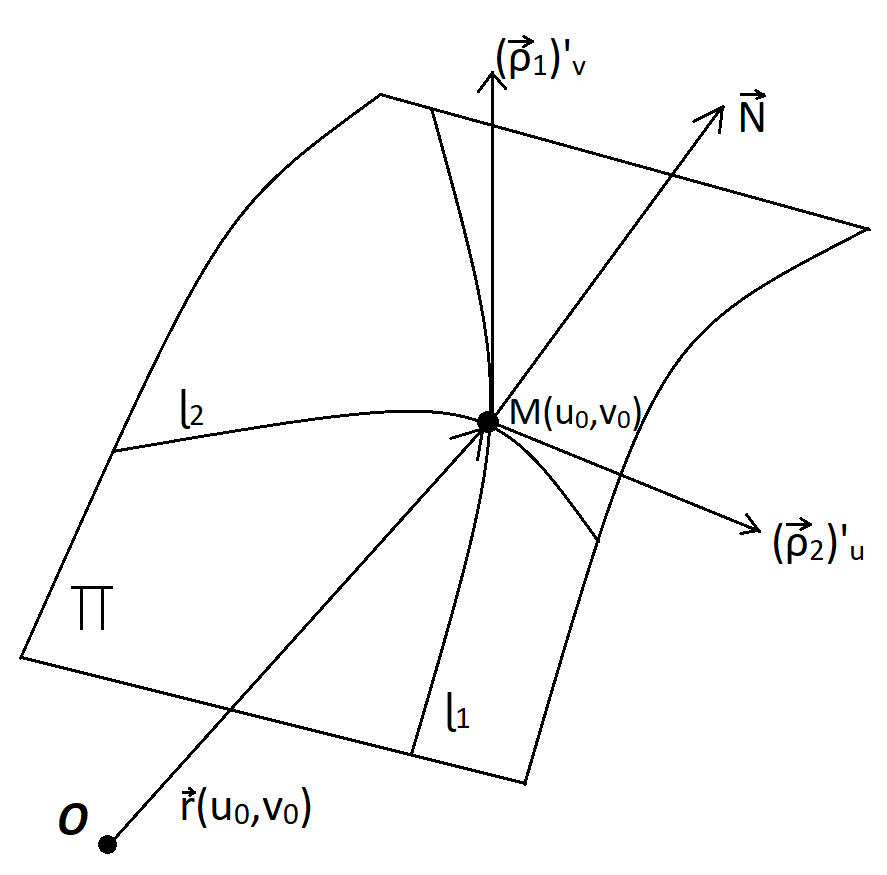
\includegraphics[scale = 0.5]{lec21_4.png}
\end{center}

Будем считать, что функции $x,\ y,\ z$ непрерывны и 
имеют непрерывные производные по $u$ и $v$, и что
\begin{equation}
\label{lec_21, num_2}
rank \dfrac{D(x,y,z)}{D(u,v)} = 
\begin{bmatrix}
x'_u & y'_u & z'_u \\
x'_v & y'_v & z'_v
\end{bmatrix} = 2.
\end{equation}

Зафиксируем какое-либо $u=u_0$. Получим вектор
$\vec{\rho_1} = \vec{r}(u_0,v)$. 
Он определяет кривую $l_1$, расположенную на поверхности $\Pi$.
Зафиксируем $v = v_0$. Получим $\vec{\rho_2} = \vec{r}(u,v_0)$. 
Он определяет кривую $l_2$.

$l_1$ и $l_2$ называют \emph{координатными кривыми} поверхности $\Pi$.

Вектор $(\vec{\rho_1})'_v$~--- \emph{касательный вектор} к кривой $l_1$:
$(\vec{\rho_1})'_v = (x'_v, y'_v, z'_v) \Big|_{(u_0,v_0)}.$
Вектор $(\vec{\rho_2})'_u = (x'_u, y'_u, z'_u) \Big|_{(u_0,v_0)}$~--- 
\emph{касательный вектор} кривой $l_2$. 

В точке $(u_0, v_0)$ определена пара касательных векторов.
Эти векторы линейно независимы в силу условия \eqref{lec_21, num_2}. 
Значит, они определяют плоскость, проходящую через $(u_0,v_0)$.
Она являестя \emph{касательной плоскостью} к $\Pi$. 
Уравнение касательной плоскости:

\[\vec{r} = \vec{r}(u_0,v_0) + (\vec{\rho_1})'_v \cdot t +
(\vec{\rho_2})'_u \cdot s = 
\vec{r}(t,s)
.\]

Вектор $\vec{N} = \pm \left[ \vec r\,'_u, \vec r\,'_v \right] = 
\pm \left[ (\rho_1)'_u, (\rho_2)'_v  \right]$~--- 
\emph{вектор нормали} к плоскости 
(его называют также \emph{вектором нормали поверхности} $\Pi$).
Он определяется с точностью до знака.

\[
\vec{N} = 
\pm \begin{vmatrix}
\vec{i} & \vec{j} & \vec{k} \\
x'_u & y'_u & z'_u \\
x'_v & y'_v & z'_v
\end{vmatrix} = 
\pm (A,\ B,\ C)
, \text{ где } A = \begin{vmatrix}
y'_u & z'_u \\
 y'_v & z'_v
\end{vmatrix},\ 
B = -\begin{vmatrix}
x'_u & z'_u \\
x'_v & z'_v
\end{vmatrix},\
C = \begin{vmatrix}
x'_u & y'_u \\
x'_v & y'_v
\end{vmatrix}
.\]

В каждой точке поверхности $\Pi$ определён вектор нормали $\pm \vec{N}$.
Если выбран какой-то конкретный знак, и в каждой точке вычислены
$(A, B, C)$, то определён вектор $\vec{N}_1 = (A, B, C)$ или
$\vec{N}_2 = (-A, -B, -C)$.
Соединим фиксированную точку поверхности с другой точкой.
Тогда, выбрав в исходной точке знак <<+>> или <<->> для вектора $\vec{N}$,
мы определим и значение вектора нормали для других точек.

Рассмотрим на поверхности $\Pi$ замкнутую кривую, 
проходящую через точку $M_0$ и
считаем, что на $\Pi$ во всех точках уже заданы конкретные направления
вектора $\vec{N}$, определённые выбранным направлением вектора нормали в точке 
$M_0$. 

Если при обходе кривой мы возвращаемся в точку $M_0$ с тем же
направлением вектора нормали, то поверхность называется \emph{двусторонней},
а если при таком обходе направление изменится на противоположное,
то поверхность называется \emph{односторонней}.

\end{document}
